%!TEX root = ../ZF-Introduction_to_Photonics-lukwidmer.tex
\mySection{Electromagnetic waves}
\vspace{2mm}
\normalsize\textbf{Wave equation for electromagnetic waves}\small
\hrule
\begin{align*}
	\nabla^2 \vv{E} - \mu_0\varepsilon_0 \frac{\partial^2 \vv{E}}{\partial t^2} = 0 \\
	\nabla^2 \vv{B} - \mu_0\varepsilon_0 \frac{\partial^2 \vv{B}}{\partial t^2} = 0 \\
\end{align*}

% TODO : This part might be unnecessairy as the plane wave already is in chapter 01
\vspace{2mm}
\normalsize\textbf{Electromagnetic plane waves}\small
\hrule
% @formatter:off
{
	\setlength{\extrarowheight}{4pt}
	\begin{tabular}{l l}
		plane wave (cplx): & \tiny$\vv{E}(\vv{r},t) = \vv{E_0}e^{i(\vv{k}\cdot \vv{r} - \omega t + \varphi)}$\small \\
		plane wave (real): & \tiny$\vv{E}(\vv{r},t) = \vv{E_0}\cos(\vv{k}\cdot \vv{r} - \omega t + \varphi)$\small  \\
	\end{tabular}\newline
}
% @formatter:on

\WhiteSpace

\mySubsection{Maxwell Equations}{3}{
	\vspace{2mm}
	\normalsize\textbf{Gauss' law for electric fields}\small
	\hrule
	\myBox {
		$$\nabla \cdot \vv{E} = \frac{\varrho}{\varepsilon_0}$$
	}
	The number of electric field lines passing through a closed surface is proportional to the electric charge enclosed by the surface is a proportional to the electric charge enclosed by the surface. An isolated positive charge generates a divergent electric field.

	\vspace{2mm}
	\normalsize\textbf{Gauss' law for magnetic fields}\small
	\hrule
	\myBox {
		$$\nabla \cdot \vv{E} = \frac{\varrho}{\varepsilon_0}$$
	}
	There is no isolated "magnetic charge". The magnetic field lines circulate back on themselves.

	\vspace{2mm}
	\normalsize\textbf{Faraday's law}\small
	\hrule
	\myBox {
		$$ \vv{\nabla} \times \vv{E} = - \partialdiff{\vv{B}}{t}$$
	}
	A time varying magnetic field generates a circulating electric field.

	\vspace{2mm}
	\normalsize\textbf{Ampère-Maxwell law}\small
	\hrule
	\myBox {
		$$ \nabla \times \vv{B} = \mu_0 \cdot \vv{J} + \mu_0 \varepsilon_0 \partialdiff{\vv{E}}{t}$$
	}
	A circulating magnetic field can be generated either by an electric current or by a time varying electric field.


}


\mySubsection{Electromagnetic wave propagation}{3}{
	\begin{myCenter}
		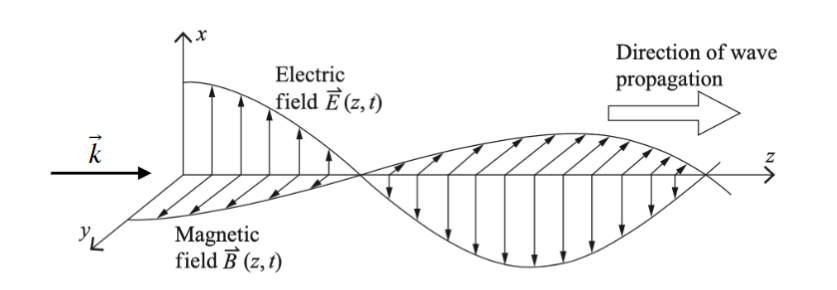
\includegraphics[align=t, width=0.6\linewidth]{01_assets/02_Electromag_wave_propagation.png}
	\end{myCenter}
	\begin{align*}
		\vv{B}(\vv{r},t) = \frac{\vv{k} \times \vv{E}}{\omega} = \frac{\vv{u} \times \vv{E}}{c}
	\end{align*}
	use: $\frac{\vv{k}}{\omega} = \frac{k}{\omega} \vv{u} = \frac{1}{c} \vv{u}$
}

\mySubsection{Permittivity \& refractive index}{3}{

	\vspace{2pt}
	% @formatter: off
	{
		\setlength{\extrarowheight}{4pt}
		\begin{tabular}{l l}
			Electron density:        & $N$                                                           \\
			Electric susceptibility: & $\chi(r, \omega) = \varepsilon(r, \omega) / \varepsilon_0 -1$ \\
			                         & $\phantom{\chi(r, \omega) }= \varepsilon_r(r, \omega) -1$     \\
			Dipole moment:           & $\vv{p} = -e\vv{x}$                                           \\
			Macroscopic polar-       &                                                               \\
			ization density:         & $-Ne\vv{x}$                                                   \\
			plasma frequency:        & $\omega_p^2 = \frac{Ne^2}{m\varepsilon_0}$
		\end{tabular}
	}
	% @formatter: on
	\newline
	\vspace{2mm}
	\normalsize\textbf{Lorenz Model}\small
	\hrule
	\tiny
	$
		\begin{aligned}
			m \frac{\mathrm{d}^2 x}{\mathrm{d}t^2} & = F_\text{driving} & + F_\text{damping}   & + F_\text{spring} \\
			                                       & = -e E_x           & - c\diff{x}{t}       & - \kappa x        \\
			                                       & = -e E_x           & - m\gamma\diff{x}{t} & - m\omega_0^2 x
		\end{aligned}
	$
	$\Rightarrow m\ddot{x} + m\gamma\dot{x} + m\omega_o^2 x = -e E_x$
	\small
	\myBox{
		$\varepsilon_r(\omega) = \varepsilon'_r + i \varepsilon''_r$ \newline
		$\varepsilon'_r(\omega)=1 + \frac{\omega_p^2(\omega_0^2-\omega^2)}{(\omega_0^2-\omega^2)^2 + \gamma^2\omega^2}$\newline
		$\varepsilon''_r(\omega)= \frac{-\gamma\omega\omega_p^2}{(\omega_0^2 - \omega^2)^2 + \gamma^2\omega^2}$
	}

	\vspace{2mm}
	\normalsize\textbf{Lorenz-Drude Model}\small
	\hrule
	\vspace{2mm}
	\begin{myCenter}
		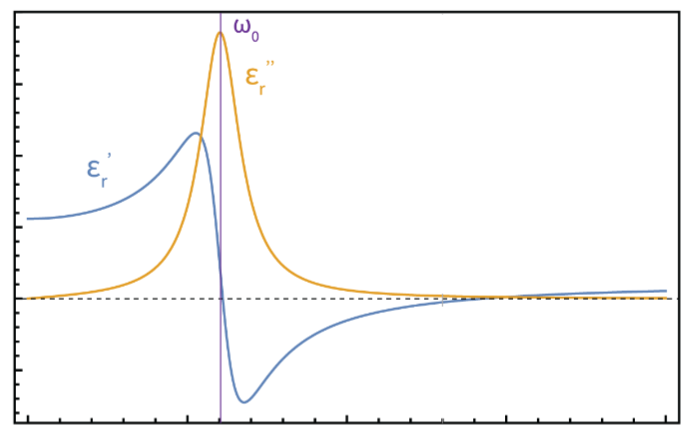
\includegraphics[align=t, width=0.45\linewidth]{01_assets/02_Electric_permittivity_dialectric.png}
		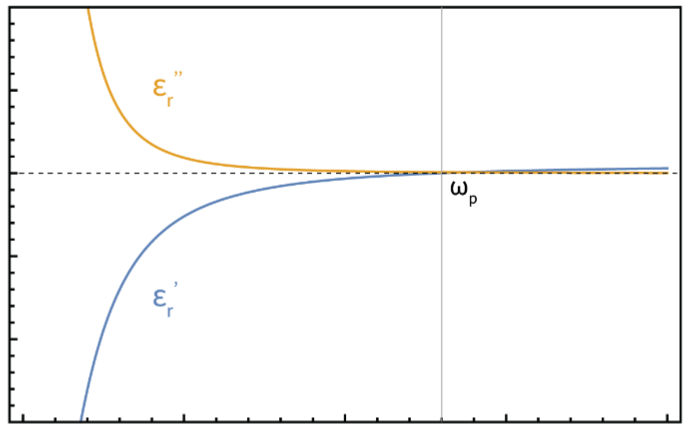
\includegraphics[align=t, width=0.45\linewidth]{01_assets/02_Electric_permittivity_metal.png}
	\end{myCenter}
	\begin{multicols*}{2}
		The model includes all terms of the Lorenz model\newline
		\columnbreak
		Electrons not bound $\rightarrow F_\text{spring} = 0 \rightarrow \omega_0 = 0$
		\textbf{Drude model:}\newline
		$\varepsilon_r(\omega) = 1 - \frac{\omega_p^2}{\omega^2 + i\gamma\omega}$
	\end{multicols*}
	\hrule
	\begin{multicols*}{2}
		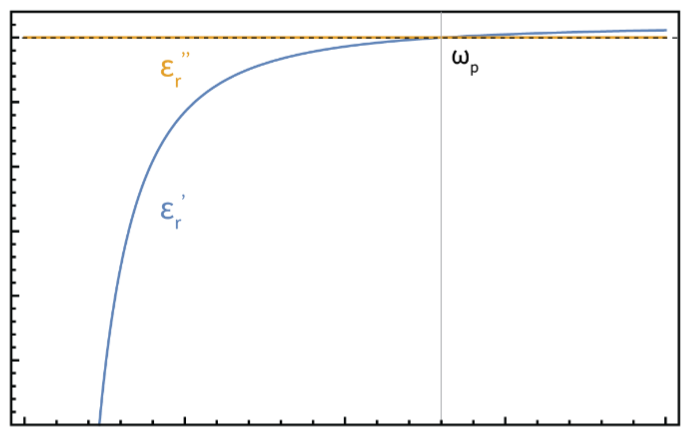
\includegraphics[align=t, width=\linewidth]{01_assets/02_Electric_permittivity_plasma.png}
		\columnbreak\newline
		Electrons not bound and no electron-phonon damping, $\omega_0 \rightarrow 0$, $\gamma = 0$.\newline
		$\varepsilon_r(\omega) = 1 - \frac{\omega_p^2}{\omega^2}$
	\end{multicols*}

	\vspace{2mm}
	\normalsize\textbf{Refractive index}\small
	\hrule
	\myBox{
		$\overline{n} = \frac{c}{v} = \sqrt{\frac{\varepsilon \mu}{\varepsilon_0 \mu_0}}$\newline
		assuming no magnetic materials\newline
		$\overline{n} = \sqrt{\frac{\varepsilon}{\varepsilon_0}} = \sqrt{\varepsilon_r}$
	}
	$$ \overline{n} = n + i\kappa $$
	$n$: refractive index \hspace{4mm} $\kappa$: extinction coefficient
	$$ \varepsilon_r' = n^2 - \kappa^2 \hspace{4mm} \varepsilon_r'' = 2 \kappa n$$
	\myBox{
		\begin{align*}
			\lambda & = \lambda_0 / n                                                                         \\
			E(x,t)  & = e^{-\alpha x} E_{0x} e^{i(kx-\omega t)} & \alpha = \frac{2\pi\kappa}{\lambda_0}       \\
			I       & = e^{-Ax}I_0 \hspace{4mm}                 & A = \frac{4\pi\kappa}{\lambda_0} = 2 \alpha
		\end{align*}

	}

}
